\section{Time Dilation and Length Contraction}
%By Matt Trawick.

\makelabheader %(Space for student name, etc., defined in master.tex)

\bigskip

\begin{wrapfigure}[5]{r}{0.35\textwidth}
\begin{center}
\vspace{-0.3in}
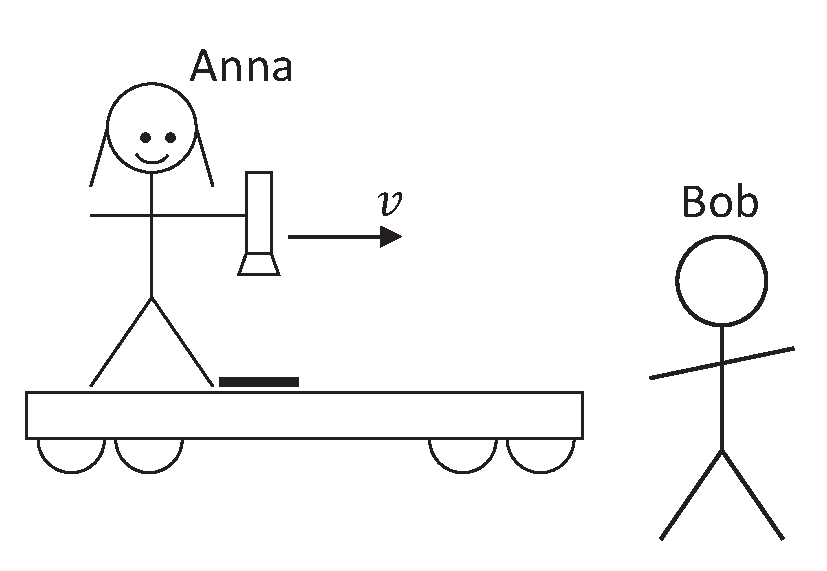
\includegraphics[scale=0.4]{time_dilation_length_contraction/anna_and_bob.eps}
\end{center}
\end{wrapfigure}

\textbf{Activity 1: Time Dilation}

%Consider the case of Anna and Bob that we talked about in class, shown in figures 2.5 and 2.6 on page 10 of Harris.  Suppose that the train is traveling with a speed $v$ such that $\gamma=1.5$.
Anna rides a train towards the east at a speed $v$ such that $\gamma=1.5$.  She turns on a flashlight, which shines onto a mirror directly below it.

\begin{enumerate}[wide, nosep]
\item If Anna measures the light's round trip time to be 6 nanoseconds, what does Bob measure?
\answerspace{0.5in}
\end{enumerate}

\begin{enumerate}[wide, nosep,resume]
\item Now Anna and Bob try a variation of the experiment.  Anna rides on the train, as before, and the train moves east again, at the same speed $v$, so that $\gamma=1.5$.  But this time Bob holds the flashlight and the mirror.  Both Anna and Bob time the round trip.  What do Anna and Bob each measure for the round trip time $\Delta t$?
\answerspace{0.5in}

\item In an experiment like what Anna and Bob are doing, the shortest measured time is called the ``proper time.''  What determines who measures the shortest time? Is it who's on the train?  Is it who holds the flashlight?  Is it who holds the mirror?
\answerspace{0.5in}

\item Write a definition of the \textit{proper time,} $\Delta t_0$, between two events.
\answerspace{0.5in}
\end{enumerate}

\begin{wrapfigure}[7]{r}{0.35\textwidth}
\begin{center}
\vspace{-0.4in}
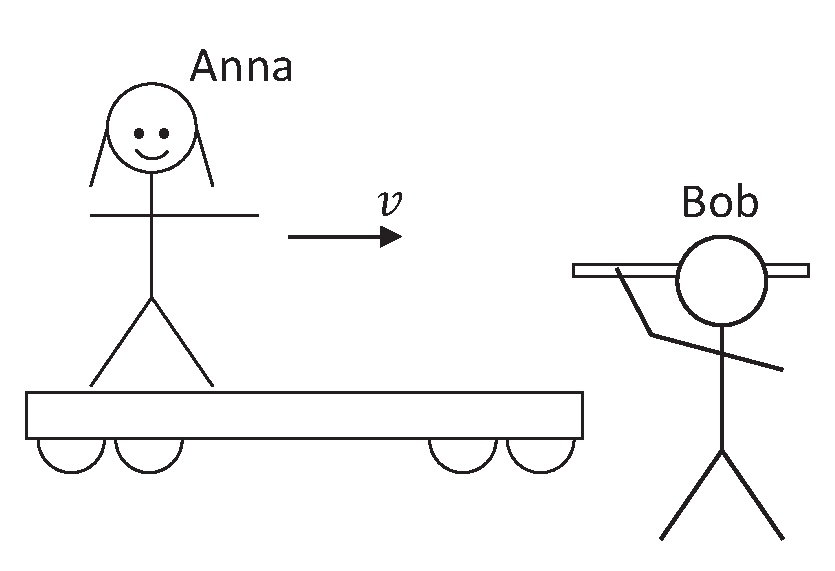
\includegraphics[scale=0.4]{time_dilation_length_contraction/anna_and_bob2.eps}
\end{center}
\end{wrapfigure}

\textbf{Activity 2: What about Length?}

Anna rides the train again at the same speed, and Bob stands on the side, holding a long rod along the direction of the train tracks.  Bob measures the rod to have length $L_0$.  Bob sees Anna traveling past at speed $v$.  Events ``A'' and ``B'' are Anna's nose being even with the left and right ends of the rod, respectively.  Bob measures the time between event A and event B as $\Delta t=L_0 ⁄ v$.  

\begin{enumerate}[wide, nosep]
\item What does Anna say is their relative speed $v$?  (Same as what Bob measures, bigger, or smaller?)
\answerspace{0.4in}
\end{enumerate}

\begin{enumerate}[wide, nosep,resume]
\item In Anna's frame, what is the time between events A and B, in terms of $\gamma$ and Bob's $\Delta t$?  (Hint: which of the two observers measures the proper time between the two events?  
\answerspace{0.4in}

\item What does Anna infer is the length $L$ of the rod?  
\answerspace{0.4in}

\item Bob's measurement, $L_0$, is the ``proper length'' of the rod.  Write a definition of ``proper length'' that highlights why Bob's measurement is different from that made in any other reference frame.
\answerspace{0.5in}
\end{enumerate}
